% Document type, font size, margin
\documentclass[11pt]{article}

% Double spacing and indentation
\usepackage{setspace}
\doublespacing
\setlength{\parindent}{0pt}

\usepackage{csquotes}

% Package required for biber/biblatex
\usepackage[
    backend=biber,
    style=numeric,
    sortlocale=de_DE,
    natbib=true,
    url=false, 
    doi=true,
    eprint=false
]{biblatex}
\addbibresource{mybib.bib}

% Set font to Arial (Tom Adcock)
% \usepackage{fontspec}
% \setmainfont[
% BoldFont=Arial Bold.ttf,
% ItalicFont=Arial Italic.ttf,
% BoldItalicFont=Arial Bold Italic.ttf
% ]{Arial.ttf}

% CHANGING FONT TO BE COMPATIBLE WITH PDFLATEX COMPILER
\usepackage[T1]{fontenc}
\renewcommand*\familydefault{\sfdefault}

% If you have Arial installed on your system, you can use it with pdflatex
\renewcommand{\rmdefault}{phv} % Helvetica as the main font
\renewcommand{\sfdefault}{phv} % Helvetica as the sans-serif font

% Given by "Example Project"
\usepackage[english]{babel}
\usepackage[a4paper,margin=20mm,marginparwidth=1.75cm]{geometry}

% Useful packages
\usepackage{amsmath}
\usepackage{amssymb}
\usepackage{graphicx}
\usepackage{tabularx}
\usepackage{subcaption}
\usepackage[justification=centering]{caption}
\usepackage{multicol}
\usepackage{fancyhdr} % Include the package for custom headers and footers
\usepackage{lipsum}   % Provides sample text. Remove this in your actual document
\usepackage{hyperref}
\usepackage{parskip}
\usepackage{fancyvrb}
\usepackage{titlesec}
\usepackage{bm}
\usepackage{pdflscape}


\setlength\parindent{20pt}

% Headers and footers
\pagestyle{fancy}     % Set the page style to fancy to apply your custom headers and footers
\fancyhf{}            % Clear all header and footer fields to start fresh
% Default header and footer settings
\fancyhead{}          % Clear all header fields
\fancyhead[L]{\leftmark} % "\leftmark" will display the current section name
\fancyfoot{}          % Clear all footer fields
\fancyfoot[C]{\thepage}  % Page number at the bottom center
\setlength{\headheight}{15pt}
\addtolength{\topmargin}{-1.6pt}  % Line width for the header rule
\renewcommand{\footrulewidth}{0pt}    % No line for the footer

% Define the null header
\fancypagestyle{nullheader}{
  \fancyhf{} % Clear headers and footers
  \renewcommand{\headrulewidth}{0pt} % No line in the header
  \renewcommand{\footrulewidth}{0pt} % No line in the footer
}

% Text that was with the HAZOP analysis
\renewcommand{\familydefault}{\sfdefault}
\usepackage{graphicx}
\usepackage{float}
\usepackage{fancyhdr}
\usepackage{multirow} 
\usepackage{lipsum}
\usepackage{array} % required for text wrapping in tables
\usepackage{lscape} 
\usepackage[table,xcdraw]{xcolor}

% Start of the document
\begin{document}
% Apply the cover page style for the cover page
\thispagestyle{nullheader}

\vspace*{2cm}
\begin{center}
\huge{\textbf{B3 Group Design Project}}\\
\huge{\textbf{Cultured Beef Production}}\\
\begin{figure}[h]
    \centering
    
\includegraphics[width=0.45\textwidth]{y0-oxford.jpg}
    \hfill
\end{figure}
\vspace*{-1cm}
{\Large Mikhail Agureev, Eunsoo Chang, William Hough, Tracey Saber}\\ % Enlarge names slightly
{\Large University of Oxford}\\ % Add some space after the university name
\vspace*{1cm}
{\large Department of Engineering Science}\\ % Separate department
{\large supervised by J. Kwan, N. Hankins, B. Nie, P. Mouthuy}\\[0.5cm] % Separate supervision line
\vspace*{0.5cm}
{\large Trinity Term 2024}

\thispagestyle{empty} % Remove page number
\end{center}
\clearpage % End of the cover page

\thispagestyle{nullheader}


\tableofcontents
\clearpage % Starts a new page after the table of contents

\thispagestyle{nullheader}
\newpage

\textbf{MAINLY TALK ABOUT WHY YOUR CHOICE LED TO A BETTER ACHIEVEMENT OF THE DESIGN OBJECTIVES.}\\

The generic structure of a technical report:

1. Introduction: Provide context, motivation, and background information

What is the big-picture problem? Why is it a problem? Who cares?

What have others done to solve the problem? What is still left to do? What did you do?

2. Methods: Explain what you did
Provide enough detail for someone else to reproduce your results.

For each aspect, the level of detail should be commensurate with the level of novelty.

3. Results: Show and explain what you found.
Provide figures and other qualitative and quantitative evidence for your conclusions.

Explain and interpret what you are showing. Not "What does the data look like?", but "What does the data mean?"

4. Discussion: Consider the implications and limitations of your results

5. Conclusions: Connect your results with the original problem.

What have you actually achieved here? What should be done next?\\

Tip 1. Emphasise results, interpretation, and discussion.

Tip 2. Technical writing needs to be precise, concise, objective, careful

Tip 3. Every sentence must: (i) make a point (ii) form a logical link between the previous sentence and the next\\
\clearpage % Starts a new page after the table of contents

\fancyhead[L]{}
\fancyhead[R]{INTRODUCTION - WILL HOUGH}
\newpage
\section{Abstract}

\subsection*{Introduction}

It’s becoming clear that the livestock farming sector is one of the main contributors to the world’s water depletion, land use, biodiversity loss and greenhouse gas emissions. Over a third of the world’s crop calories are used as animal feed, and only a third of those feed calories end up contributing to the human diet. [https://iopscience.iop.org/article/10.1088/1748-9326/8/3/034015] With trends in global consumption and production of meat growing, the impacts of livestock farming are set to grow.
Alternative protein developments aim to substantially reduce the impact of feeding the human and domesticated animal population of the world by substituting the billions of animals grown and slaughtered every year with an alternative. There are significant developments in the plant-based, microbial, and fermented protein research, but we focus on evaluating the viability of directly substituting reared and slaughtered cattle with commercially cultured beef. 

% \begin{figure}[h]
%     \centering
%     
\includegraphics[width=0.75\textwidth]{will/example-image.jpg}
%     \hfill
%     \caption{An example image \citet{E-Cannon2022}}
%     \label{fig:example-image}
% \end{figure}

\subsection*{Summary}

Whilst shifting crop use away from animal feed could feed an additional 4 billion people and reduce global Green House Gas emissions by about a tenth, our venture proposal wouldn’t be profitable in today’s political and economic climate. [https://iopscience.iop.org/article/10.1088/1748-9326/8/3/034015] [https://www.sciencedirect.com/science/article/pii/S0377840111001933 MAKE SURE TO ACCOUNT FOR INCREASE IN CROP CONSUMPTION]
Unless commissioned by a special interested party – the outgoings and capital cost, along with risk associated with such a new, volatile and saturated market – mean that the proposal is unlikely to work better than other protein alternatives. If policies were introduced that reduced the subsidies on traditionally farmed meat and moved them to cultured meat, then our proposal might gain more traction to feed demand as our prices ease. [https://www.oxfordmartin.ox.ac.uk/blog/meat-and-dairy-gobble-up-farming-subsidies/]

% Example equation \ref{eq:example-equation}.

% \begin{equation}
%     beef_{moo} = fear^{10}
%     \label{eq:example-equation}
% \end{equation}

% Example list:

% \begin{itemize}
%     \item \(\bm{X} \in \mathbb{R}^{n \times p}\), a matrix containing the scrutinised data-points $\bm{x} \in \mathbb{R}^{p}$ from each sample,
%     \item \textit{regression\textunderscore targets}, known as $\bm{\bar{y}}\in \mathbb{R}^n$, is a vector containing the regression targets for the samples (individually known as $\Bar{y}$), and
%     \item \textit{class\textunderscore labels} $\in \{1,\dots,p\}$ which keeps track of which Gaussian each sample came from (a target for classification).
% \end{itemize}

% Example table \ref{table:1}

% \begin{table}[!ht] % the [h] forces the table to be "here". This is quite a short document so LaTeX struggles to find a nice arrangement for the floats! Not normally needed
%     \begin{center}
    
%         \begin{tabular}{|l|c|c|} 
%             \hline
%             \textbf{learning\_rate} & \textbf{mse\_train} & \textbf{mse\_val} \\ 
%             \hline
%             1e-05&1.1254&1.1747\\
%             \hline
%             0.0001&0.31296&0.3012\\
%             \hline
%             0.001&0.095492&0.088045\\
%             \hline
%             0.01&0.046835&0.052905 \\
%             \hline
%             0.1&0.046534&0.052771\\
%             \hline
%             1&NaN&NaN \\
%             \hline
%         \end{tabular}
%         \caption{Table of Mean Squared Difference from different learning rates.}
%         \label{table:1}
            
%     \end{center}
% \end{table}

% Example aligned equation:

% \begin{align*}
%     \mathcal{L}_c &= -ylog(\bar{y}) - (1-y)log(1-\bar{y})\\
%     &= ylog(1+e^{-\bm{\hat{x}^T\theta}})-(1-y)log(\frac{e^{-\bm{\hat{x}^T\theta}}}{1+e^{-\bm{\hat{x}^T\theta}}})\\
%     &=(y-y)log(1+e^{-\bm{\hat{x}^T\theta}})-(1-y)log(e^{-\bm{\hat{x}^T\theta}})+log(1+e^{-\bm{\hat{x}^T\theta}})\\
%     &=(1-y)\bm{\hat{x}^T\theta}+log(1+e^{-\bm{\hat{x}^T\theta}})\\
%     \Delta_{\bm{\theta}}\mathcal{L}_c &=(1-y)\bm{\hat{x}}-\frac{e^{-\bm{\hat{x}^T\theta}}}{1+e^{-\bm{\hat{x}^T\theta}}}\bm{\hat{x}}\\
%     &=(1-y)\bm{\hat{x}}-(1-\bar{y})\bm{\hat{x}}\\
%     &=\bm{\hat{x}}(\bar{y}-y)
% \end{align*}

% END OF TEMPLATE

\fancyhead[L]{}
\fancyhead[R]{CELL SELECTION - WILL HOUGH}
\newpage
\section{Cell Selection}

\subsection{Introduction to Cells}

Our final product is a combination of muscle cells and oleogel-based fat substitute [https://www.nature.com/articles/s41467-023-38593-4]. Of the three muscle cell types (myocytes) found in vertebrates, beef is composed of skeletal muscle cells [https://www.ncbi.nlm.nih.gov/pmc/articles/PMC5167519/]. These cells can be derived from myoblasts through a process known as myogenesis, explained further in [SECTION DIFFERENTIATION]. 

[https://www.researchgate.net/figure/Myoblast-differentiation-Activated-satellite-cells-are-called-myoblasts-They-express_fig25_231588877] OR USE TRACEY’S FIGURE 4

The definition of a myoblast is “an undifferentiated cell capable of giving rise to muscle cells” [https://www.merriam-webster.com/dictionary/myoblast], which includes many different types of stem cells. When designing our cultured meat process, we need ensure our primary cells are suitable for both the process and final product. 

Myosatellite cells are the mode cell type used in industry, 23.1\% of 40 companies. [GFI-APAC-cell-line-survey-report-19-June-2023]

\subsection{Stem Cells}
We considered the following stem cell types for seeding our bioreactors:

\subsubsection*{Skeletal Muscle Stem Cells (Myosatellite)}
Under resting condition myosatellite cells are quiescent [dormant] and reside under the basal lamina [https://en.wikipedia.org/wiki/Basal_lamina] of the myofiber [https://www.sciencedirect.com/science/article/pii/B9780124160224000068?via\%3Dihub]. The overall myogenic differentiation pathway includes the activation of quiescent satellite cells, commitment to differentiation and proliferation, fusion to form myotubes, and ultimately maturation into myofibers.

\subsubsection*{Mesenchymal Stem Cells}
Mesenchymal stem cells (MSCs) are stromal cells that can self-renew. They are also capable of multilineage differentiation. MSCs can be isolated from a variety of tissues, such as umbilical cord, endometrial polyps, menses blood, bone marrow, adipose tissue, etc. [https://pubmed.ncbi.nlm.nih.gov/21396235/]. One of the major challenges is to elucidate the mechanisms of differentiation, mobilization, and homing of MSCs, which are highly complex.

\subsubsection*{Embryonic Stem Cells}
Embryonic stem cells (ESC) are obtained from the inner cell mass of the blastocyst and are associated with tumorigenesis [https://pubmed.ncbi.nlm.nih.gov/21396235/]. Embryonic stem cells are pluripotent meaning they can differentiate into all derivatives of the three primary germ layers. ESCs are capable of self-renewal in conditions that prevent differentiation and clumping. [https://www.science.org/doi/10.1126/science.282.5391.1145] [https://www.cell.com/cell/fulltext/S0092-8674\%2803\%2900847-X ]. ESCs have a shortened G1 phase and thus divide very frequently, allowing the cells to multiply quickly. ESCs have ethical considerations as harvesting embryonic stem cells usually necessitates destroying the embryo from which those cells are obtained.

\subsubsection*{Induced Pluripotent Stem Cell (iPSC)}
iPSCs can be obtained by reprogramming differentiated somatic cells. The genetic engineering required is high-cost due to its sensitivity, however base cell biopsy samples are easy to gain. Performance characteristics are similar to ESCs. [https://www.ncbi.nlm.nih.gov/pmc/articles/PMC3347549/] 

\subsection*{Other Cell Types}
The following cell types may be useful:

\subsubsection*{Fibroblast}
Fibroblast cells are used in the production of the extracellular matrix that can be used to provide texture to the meat. They can replicate indefinitely in vitro and are found in many parts of the body including skin. [https://www.ncbi.nlm.nih.gov/books/NBK26889/]

\subsubsection*{Adipocyte}
Adipocytes are the energy storage mechanism of the body, also known as fat cells. They are derived from Mesenchymal Stem Cells via adipogenesis. [https://www.ncbi.nlm.nih.gov/books/NBK555602/]

\begin{figure}[h]
    \centering
    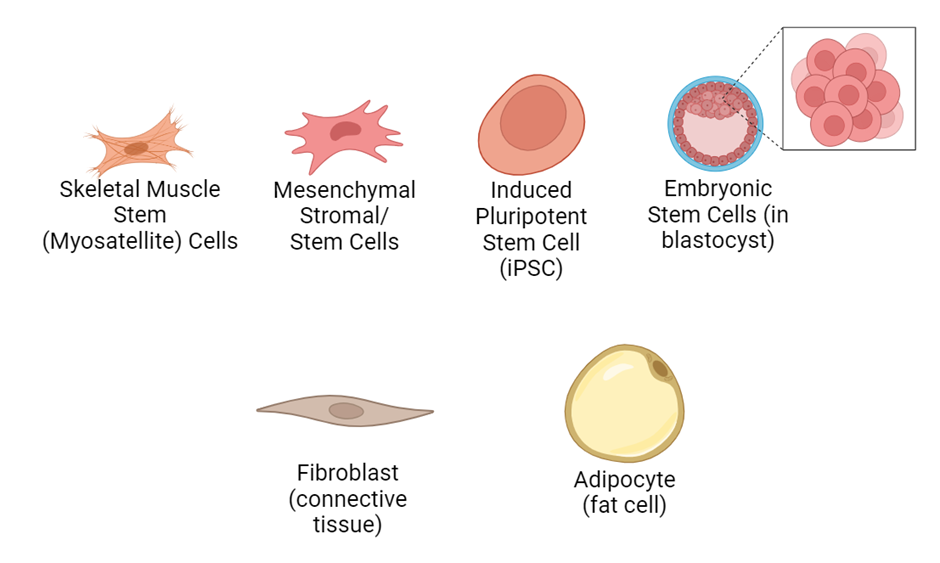
\includegraphics[width=0.75\textwidth]{will/w2i-cell-types.png}
    \hfill
    \caption{Cell types discussed, made in Biorender}
    \label{fig:cell-types}
\end{figure}



\fancyhead[L]{}
\fancyhead[R]{MICROCARRIERS - WILL HOUGH}
\newpage
\section{Control systems}

\subsection{Introduction}

Scaffold Selection
Skeletal muscle cells are themselves adherent – they’re named after the fact they adhere to bones. In vivo, cells exist within an extracellular matrix of proteins and proteoglycans. Complex interactions known as mechanotransduction occurs between the stiffness of the matrix and the cells within it. These interactions are governed by integrins and lead to downstream signaling that can affect cell polarity, migration, and differentiation.
During the proliferation phase, we grow anchorage-dependent stem cells in large scale bioreactors. The non-native environment can lead to anoikis if cells are not adapted to suspension growth, tricked into via molecules such as Rho Kinase inhibitors to be anchorage independent or grown as spheroids. We can bypass activation of anoikis in suspension by using a scaffold that enables cellular adherence.
Another factor to consider would be the materials used in our scaffolds. We need to ensure they meet our primary directives and the goals of the group.
 
[https://gfi.org/wp-content/uploads/2023/01/Figure-4-Scaffold-Types_v1.pdf]
Microcarriers
Microcarriers are small spherical structures that mimic extracellular matrix characteristics to allow cellular attachment. Whilst there are other scaffolding techniques available, microcarriers have the advantage of providing a large surface area to volume ratio, permitting high densities of cells in the proliferation phase.
[https://gfi.org/science/the-science-of-cultivated-meat/deep-dive-cultivated-meat-scaffolding]
[https://www.mdpi.com/2304-8158/10/12/3116]
 
Figure 1"C:\Users\will\OneDrive - Nexus365\Eng\Year3\B3\Group Work\Resources and Documents\External\231016 Ivy Farm Industry Talk Oxford - Share.pdf"
[https://www.sciencedirect.com/science/article/pii/S0268005X22001527]
Porous Scaffolds
Porous scaffolds try to mimic the extracellular matrix of a tissue. Generally, porous scaffolds allow adhesion, mass transport, migration and cell distribution. To accommodate this, they need to be biocompatible to avoid an immune response and they can enhance tissue growth by being bioactive.
Typical scaffold structures can be foams or lattices. If foamed, they need a manufacturing process that ensures the interconnectivity of pores and pore size, to prevent hypoxic conditions due to stagnation. Manufacturing processes like this are complex and don’t guarantee performance.
[https://pubs.acs.org/doi/10.1021/acsabm.2c00740]
Hydrogels
Hydrogels are made up of three-dimensional networks of crosslinked hydrophilic polymers. They can absorb large amounts of fluids, up to several thousand \%, and readily swell without dissolving. When swollen they resemble living tissues in texture – rubbery and soft.
[https://www.ncbi.nlm.nih.gov/pmc/articles/PMC3963751/]
Chitosan and alginate-based hydrogels meet the biocompatible requirements needed to prevent an immoresponse from our cultured cells. [https://onlinelibrary.wiley.com/doi/abs/10.1002/app.10137]
 
Figure 2https://www.ncbi.nlm.nih.gov/pmc/articles/PMC3963751
Hydrogels can be obtained by various methods – most commonly physical crosslinking, chemical crosslinking, free radical polymerisation and irradiation crosslinking [see fig below]
 
Figure 3 https://www.ncbi.nlm.nih.gov/pmc/articles/PMC3963751
[https://link.springer.com/article/10.1007/s10856-019-6318-7 and "C:\Users\will\OneDrive - Nexus365\Eng\Year3\B3\Group Work\Project Collaboration\Will\s42242-021-00165-0.pdf"]
Additional techniques
3D Printing and other additive techniques
3D printing can be used to print either the product, allowing greater control over the composition and texture, or the ECM-like porous scaffold used in cell proliferation, allowing us to print a fluid-modelled growth-structure that we’re certain allows proper perfusion. Additive techniques, however, decrease cell viability after micro extrusion by around 40-86\% due to extrusion pressure and shear stress. The process requires specialist, precision, equipment – increasing complexity, maintenance, and capital costs. 
 
Figure 4 "C:\Users\will\OneDrive - Nexus365\Eng\Year3\B3\Group Work\Project Collaboration\Will\s10856-019-6318-7.pdf"
Fiber Scaffolds
Much like porous scaffolds, we can make cell supporting structures using microfibres. Cellulose fibres meet our criteria for biocompatibility, mechanical strength and reactive surfaces for protein binding, however very few studies have looked into the application of cellulose microfibers as a scaffold in cell culturing due to the absence of an intrinsic 3-D structure. Use of gelatin may provide the needed 3-D architecture – gelatin is collagen derived and is nonimmunogenic, inexpensive and biodegradable. Research shows that cellulose microfiber/gelatin composites containing up to 75\% cellulose fibres are more capable of withstanding mechanical loads than gelatin alone.
[https://www.sciencedirect.com/science/article/pii/S1742706109005777]
Gelatin is produced through partial hydrolysis of collagen, which is typically from bovine or porcine sources. This means that whilst cellulose itself is plant based, cellulose fiber scaffolds don’t meet our requirements for reducing reliance on existing animal agriculture and slaughter.
[https://www.sciencedirect.com/topics/chemistry/gelatin]
Additional factors
Typically, scaffolds are used in the proliferation process, after which the cells are harvested using trypsin, accutase and/or sonication. [https://pubmed.ncbi.nlm.nih.gov/30504375/][ https://www.nature.com/articles/s41598-022-09605-y] However, harvesting puts the cells at risk of death – reducing yield – and adds further operations to an already complex process. If we consider the texture and composition of the final product, we know that since techniques for growing fibrous muscle or spatially patterned 3D substrates haven’t developed yet, the structure of our final product will be a homogenised microtissue structure – as seen in ground beef. To add texture to the homogenised microtissues we need a binding/aggregating agent, which is often added to the cells after they are harvested from their proliferation scaffold.
If we can find a proliferation scaffold that can stay in the final product and increase the aggregate size, we remove the need for harvesting and secondary scaffold addition. This will be a significant improvement on the product and thus should be weighted as such in our multi-criteria analysis. If we do manage to find something suitable, we note we’ve removed the option of recycling our proliferation scaffold, which means we need to ensure we have a well optimised scaffold manufacturing process.  

Figure 5 Structured Final Beef Burgers  https://static-content.springer.com/esm/art\%3A10.1038\%2Fs41467-023-38593-4/MediaObjects/41467_2023_38593_MOESM6_ESM.mp4

Microcarrier Materials and Manufacturing [https://www.sciencedirect.com/science/article/pii/S0268005X22001527]
Materials
Chitosan (Av. MW 890,000 Da, degree of deacetylation: 93\%) was purchased from Glentham Life Sciences (Wiltshire, UK). Sodium tripolyphosphate (TPP) was purchased from Alfa Aesar (Ward Hill, MA, USA). Bovine Achilles tendon collagen and porcine gastric pepsin were purchased from Sigma Aldrich (Rehovot, Israel). Epigallocatechin gallate (EGCG) was supplied by Healthy origins (Pittsburgh, PA, USA).
Substitute tendon collagen for biomimetic plant based collagen.
[https://go.gale.com/ps/i.do?id=GALE\%7CA776940777&sid=sitemap&v=2.1&it=r&p=HRCA&sw=w&userGroupName=anon\%7E8cbba7f9&aty=open-web-entry]
Substitute pepsin with animal free pepsin. [https://theeverycompany.com/news/pepsin]
Manufacturing of cell microcarriers
A 2\% chitosan (CS) solution in 0.2M acetic acid was electrosprayed through a 27G needle into a 2\% TPP crosslinking solution. Alternatively, a solution of 1\% collagen (COL) in 0.5M acetic acid was prepared using 0.1\% pepsin and electrosprayed into a 1\% EGCG crosslinking solution. In the case of composite microcarriers, chitosan and collagen solutions were mixed at a mass ratio of 90:10, respectively, to achieve a final polymer concentration of 2\%. The spray distance, applied voltage, flow rate, and polymer concentration were optimized according to Tables S1 and S2. The obtained MCs were sterilized using 70\% ethanol and then washed 2 times for 60 min in double distilled water, once in phosphate buffer saline (PBS), and once in a growth medium before seeding the cells.
For the seeding, microcarriers were incubated with the cells at 37 °C and 5\% CO2 overnight in a ratio of 5000 cells/cm2. The seeding area was determined as S = 4 × π × R2 × N, where S is the seeding area, R is the radius of MCs, and N is the number of MCs.
Optimal size being spherical microparticles with a smooth surface and narrow size distribution of 571 ± 66 μm diameter.

Bacterial collagen substitute [https://www.frontiersin.org/articles/10.3389/fchem.2014.00040/full]

Plant collagen [https://www.sciencedirect.com/science/article/pii/S0268005X22001527#bib45]

Muscle cell @ 3.5e-13kg [Mike ref]

collagen/chitosan scaffold aerogels @ 0.0468 g/cm3 = 46.8kg/m3  [https://www.sciencedirect.com/science/article/pii/S0928493118306295]
For the seeding, microcarriers were incubated with the cells at 37 °C and 5\% CO2 overnight in a ratio of 5000 cells/cm2. The seeding area was determined as S = 4 × π × R2 × N,

The addition of a low EGCG concentration (0.02\%) resulted in spherical microparticles with a smooth surface and narrow size distribution of 571 ± 66 μm diameter. This means each microcarrier has a 
volume of 97.48e-12m3, and thus a 
mass of V*rho = 4.562e-9kg.
A surface area of 4*pi*r^2 = pi*d^2 = 1.0243e-6 m2

Our starting density is 50e6 cells per m2 of microcarrier surface area. This is 51.2 cells per microcarrier. [https://www.sciencedirect.com/science/article/pii/S0268005X22001527#appsec1:~:text=2.5.\%20Cell-,seeding,-and\%20cultivation\%20on]
However, if we go with the later studied seeding density of 9000 cells per cm2 or 90e6 cells per m2 we get a seeding of 92.187 cells per microcarrier.
[https://www.nature.com/articles/s41467-023-38593-4#MOESM4:~:text=Cell\%20seeding-,Edible,-cell\%20microcarriers\%20were]

Our final amount of meat each cycle is about 100kg
At 20\%m/m of fat this leaves 80kg of cells + microcarriers.
Optimistic cell densities achieved in production STRs are around 2e6cells/mL = 2e12cells/m3. [https://www.frontiersin.org/articles/10.3389/fsufs.2019.00044/full]
With random packing of equal spheres we get approx. 63.5\% of space taken up.
This means that in a 1m3 space we can pack 1/(97.48e-12m3/63.5\%) = 6.514e9 microcarriers/m3
This gives a microcarrier to cell ratio of 1:307 or roughly 1:300.
This gives a microcarrier to cell mass ratio 1:0.2355 or 4.246:1
Thus, of our 80kg, we have 15.25kg of raw cells and 64.75kg of microcarriers.

Further attempts to reduce the collagen concentration in the MC led to a decreased cell viability: (Fig. S3), hence the 90:10 CS/COL-MCs were used in our following studies.
 
Figure S3. Viability of C2C12 cells cultured on CS/COL-MCs produced using different ratios of chitosan to collagen. 
https://www.sciencedirect.com/science/article/pii/S0268005X22001527



\fancyhead[L]{}
\fancyhead[R]{MEDIUM - TRACEY SABER}
\input{tracey/T1-Medium}

\fancyhead[L]{}
\fancyhead[R]{PROLIFERATION SEED - TRACEY SABER}
\input{tracey/T2-Proliferation}

\fancyhead[L]{}
\fancyhead[R]{OXYGENATION - WILL HOUGH}
\newpage
\section{Control systems}

\subsection{Introduction}
Oxygenation
Our process revolves around the growth and harvesting of bovine cells. Preventing cell death and enabling growth in mammalian cells means we need to ensure they’re able to respire. The body does this with the use of the bloodstream – oxygen enters the lungs and binds to the haemoglobin on red blood cells, which are then pumped around the body through a network of vessels to oxygenate our cells. This prevents necrosis and allows cells access to energy via their mitochondria for work and division.
Since we’re using a [batch-fed] bioreactor, we can use the culture media as our vehicle for oxygen, as we know all live cells have access to the medium thanks to cell requirements. We also need to control the CO2 content of the medium at a reasonable, [and our gas cycling could be just the way to extract it.]
Medium Oxygenation Methods
Purified Oxygen
Oxygenation can be done with air or oxygen. 
If using purified oxygen, much less gas is needed but it’d have to be purchased or refined on site – which increases operating & capital cost, complexity, and maintenance. There are a few different methods for obtaining oxygen.
-	Electrolysis – relatively high cost, studies show it can be viable with photovoltaic cells if we sell the hydrogen for 10eur/kg, the oxygen is worth 3eur/kg. [https://www.sciencedirect.com/science/article/pii/S0306261921012964]
-	Purchase cylinders @ £41 ex. VAT for 85kg of O2, or 50p/kg [https://www.boconline.co.uk/shop/en/uk/gas-a-z/oxygen/oxygen-cylinder-medical-grade-compressed-gas]
-	PSA/VPSA involves separating air into its constituent components by means of adsorption. In other words, the gas molecules bind with adsorbent material at different rates depending on the pressure. This allows operators to single out one particular gas from air. [https://www.linde-engineering.com/en/images/Oxygen\%20generation.\%20By\%20Vacuum\%20Pressure\%20Swing\%20Adsorption._tcm19-416454.pdf] Refining oxygen from air using vapour pressure swing adsorption has promise for higher consumption tasks such as in hospitals, but studies and simulations show that PSA plants are not viable are not economical at low capacity – quotes estimate prices of $115900-2228000. [https://wobogroup.en.made-in-china.com/product/ldIfpNxPXsYe/China-Best-Price-95-Purity-Oxygen-Vpsa-Plant-Gas-Generation-Equipment.html] [https://www.ncbi.nlm.nih.gov/pmc/articles/PMC10993950/] 
Figure 1https://www.wobogroup.com/product/VPSA-Oxygen-GeneratorsO2.html
Air
If using air, other gases and pollutants within the air need to be tracked/filtered, in particular CO2 and carcinogens. This can be handled with filtering and purification and is typically the method that we see in cultured meat scientific papers due to its simplicity and availability. [https://www.nature.com/articles/s41467-023-38593-4]
Gas Sparging
Gas spargers are usually placed at the bottom of the reactor, where small holes emit small bubbles of gas from the supply. The bubble path takes them through the medium, oxygenating the liquid by diffusion with the additional benefit of bubbled mixing.
Bubbled aeration can produce foam on the surface of the culture; thus a foam control system is needed to prevent excessive foam buildup as foam disrupts the proper suspension of microcarriers.
 
Figure 2 Gas sparging bubbling, extract from https://static-content.springer.com/esm/art\%3A10.1038\%2Fs41467-023-38593-4/MediaObjects/41467_2023_38593_MOESM4_ESM.mp4
 
Figure 3https://static-content.springer.com/esm/art\%3A10.1038\%2Fs41467-023-38593-4/MediaObjects/41467_2023_38593_MOESM1_ESM.pdf
 
Headspace Overlay
Some studies use an overlay to pump gas into the headspace of the bioreactor to allow diffusion into the cell media from above. This has been shown to be effective with filtered air as the pumped gas. [https://www.nature.com/articles/s41467-023-38593-4]
Since the headspace overlay method has proven effective, simple and affordable – this is the method we have chosen for our process. We can measure oxygen transfer using Oxygen Quotient [https://www.alicat.com/monitor-outgassed-material-in-bioreactor-headspace/] and use researched methods from the AIChE to enhance oxygen mass transfer [https://aiche.onlinelibrary.wiley.com/doi/epdf/10.1021/bp00015a010]. We’ll use a pump and filter system that shouldn’t cost more than an estimate of [£2000], but it’s important to get a quote should we need a precise number [estimate references?].
 


\fancyhead[L]{}
\fancyhead[R]{CONTROL SYSTEMS - EUNSOO CHANG}
\newpage
\section{Control systems}
\vspace{-3mm}
\subsection{Introduction}
\vspace{-3mm}

% 4 pages given, 8 sections in total.
% Each section should be roughly 1/2 page long.

% - (I) What is a bioreactor control system?

Homeostasis, defined as the internal regulatory functions of the body to maintain certain conditions constant~\citep{E-Guyton2006, E-Aging2022}, is extremely crucial to living organisms. For example, for humans, the blood pH outside the range between 7.35 and 7.45 can cause death \cite{E-Donaldson2013}. In addition to its significance in maintaining an existing life, homeostasis has great importance in creating a new life: Mammalian cell culture.

In a bioreactor, homeostasis can be achieved by solving the classical problem of tracking the reference signal $r(t)$ in control theory, as shown in Figure \ref{figure:E-1-1-control-system}. A thoroughly designed bioreactor and its constituent control systems will lead to better achievement of the design objectives, which are: (i) How can one achieve the production rate of 100 kg/month? (ii) How can one produce a better quality of meat?

The design of the control system mainly answers the latter question. The former question is rather answered through the overall process diagram, number and sizes of bioreactors, mass inflows and outflows, so will not be tackled in this chapter. Bioreactor control, however, addresses the formation and maintenance of the optimal environment to produce the best quality of meat. Thus, in this chapter, the design of temperature (T), dissolved oxygen (DO) and acidity (pH) control systems are discussed.

\begin{figure}[h]
    \centering
    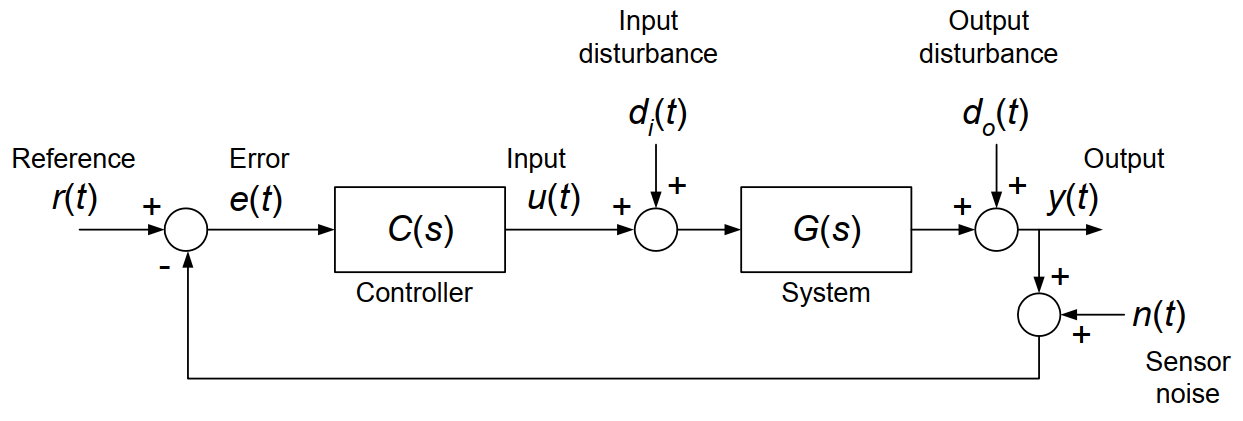
\includegraphics[width=0.75\textwidth]{eunsoo/E-1-1-control-system.png}
    \hfill
    \caption{A schematic of a negative feedback control system \citet{E-Cannon2022}}
    \label{figure:E-1-1-control-system}
\end{figure}

\vspace{-10mm}
\subsection{Temperature control}
\vspace{-3mm}
\subsubsection{Introduction}

% - (I) why consider control systems for temperature?

The body temperature of beef cattle should be maintained at $39.6 \pm 0.1 ^{\circ} C$ \cite{E-Gaughan2014}. To do so, different physical setups of the heat exchanger around the bioreactor will be compared to find the optimal one. Differential equations will be constructed to derive the plant transfer function. Design criteria will be posed with appropriate justification. Different control strategies will be compared to find the optimal one. The design criteria introduced will be used to find control parameters. MATLAB simulations will be used to confirm the validity of the step and impulse responses.

\subsubsection{Methods}

% - (M1) the physical structure of the temperature control system and justification

Various types of heat exchangers used to control the heat in and out of the bioreactor are shown in Figure \ref{figure:E-1-2-heat-exchangers}. The best design choice is (a), the jacketed bioreactor. The logic is as follows: (c) and (d) have the heat exchange inside the bioreactor, causing an intervention in the rotational pathway of the impeller used to stir the meat, and thus adding unnecessary complexity to the design to avoid this; (e) involves taking the meat out of the bioreactor, which firstly may harm the meat cells by pumping and pressurising them above the maximum stress that they they can resist, and secondly has a potential issue of fouling in the pump. One is now left with (a) and (b), but for better heat transfer it is more efficient for the working fluid to cover the entire bioreactor, and for more evenly distributed heat transfer it is better if the inlet and the outlet temperatures of the heat exchanger do not vastly differ. Hence, (a) is the best option.

\begin{figure}[h]
    \centering
    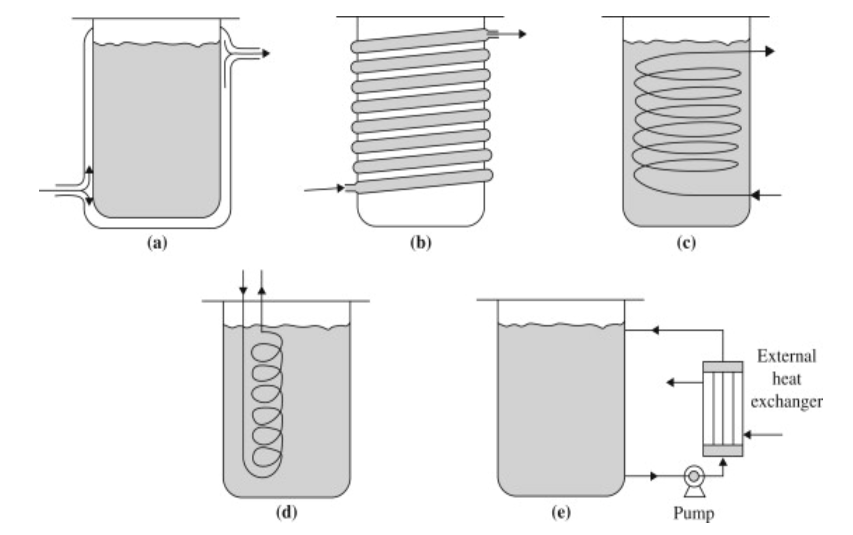
\includegraphics[width=0.5\textwidth]{eunsoo/E-1-2-heat-exchangers.png}
    \hfill
    \caption{Heat exchanger configurations for a bioreactor \cite{E-Doran2013}}
    \label{figure:E-1-2-heat-exchangers}
\end{figure}

\vspace{-5mm}
Theoretically, the heat exchanger's working fluid temperature $T_{fluid}$ controls the bioreactor's internal temperature $T$. Practically, the observer is implemented using a temperature sensor, and the controller is implemented digitally using a computer system, as shown in Figure \ref{figure:E-1-3-digital-control-system}.

\begin{figure}[h]
    \centering
    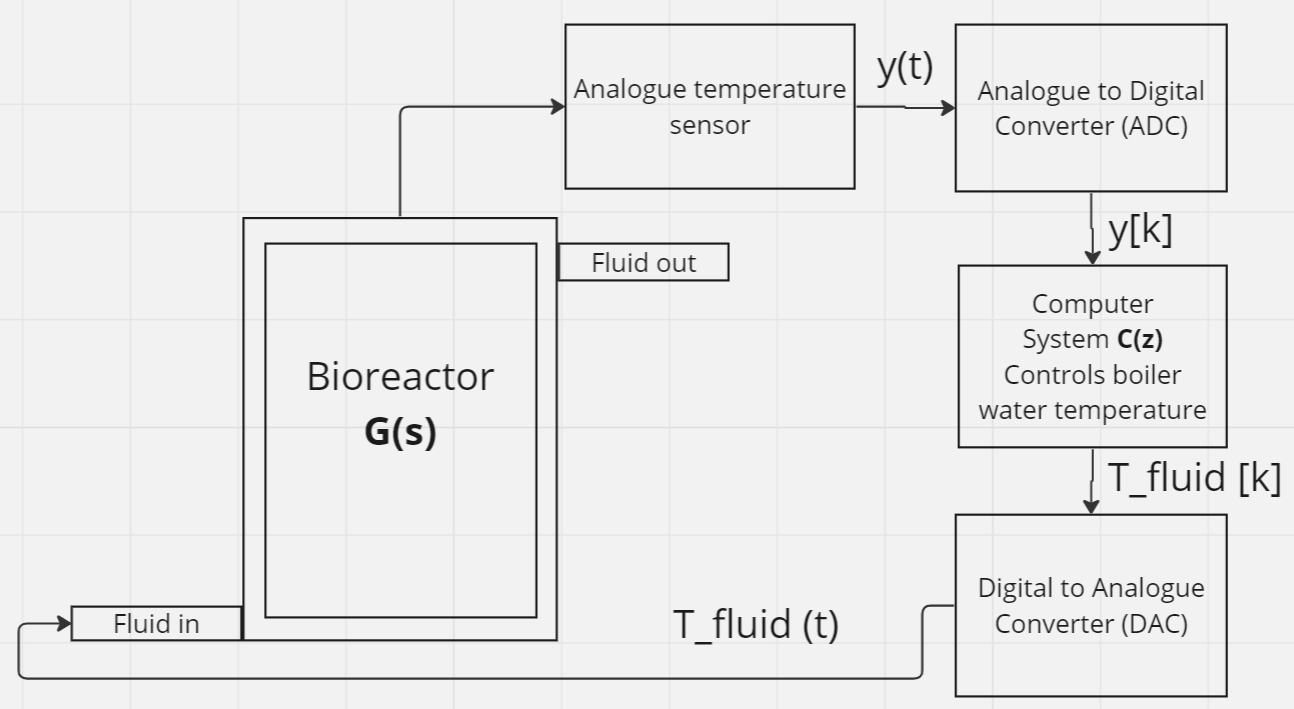
\includegraphics[width=0.6\textwidth]{eunsoo/E-1-3-digital-control-system.png}
    \hfill
    \caption{Practical implementation of the control system}
    \label{figure:E-1-3-digital-control-system}
\end{figure}

\newpage

% - (M2) the mathematical model and transfer function derivation for temperature control

The dynamics over time of temperature ($T$) can be described via the energy balance equation, where $\rho$ is the wet cell density, $V$ is the volume of the bioreactor, $c_p$ is the specific heat capacity, $Q_{met}$ is the metabolic heat generation rate, $h$ is the heat transfer coefficient and $A$ is the area of the bioreactor.

\vspace{-5mm}
\begin{equation}
    \rho V c_p \frac{\partial T}{\partial t} = Q_{met} V - hA(T-T_{fluid})
\end{equation}

The change of variables to perturbations $\Delta T = T(t) - T_{ss}$ and $\Delta T_{fluid} = T_{fluid}(t) - T_{fluid, ss}$ leads to Equation \ref{equation:E-temp-2}. During the entire culturing period ($t>0$) the steady-state assumption ($\frac{\partial \Delta T}{\partial t} = 0$, $\Delta T \approx \Delta T_{fluid} \approx 0$) can be made because otherwise the cells will die due to the violence of homeostasis. This leads to Equation \ref{equation:E-temp-3}. Substituting Equation \ref{equation:E-temp-3} into Equation \ref{equation:E-temp-2} and taking the Laplace transform leads to the desired transfer function, as shown in Equation \ref{equation:E-temp-4}.

\vspace{-5mm}
\begin{equation}
    \rho V c_p \frac{\partial \Delta T}{\partial t} = Q_{met} V - hA(T_{ss} - T_{fluid, ss}) - hA(\Delta T - \Delta T_{fluid})
    \label{equation:E-temp-2}
\end{equation}

\vspace{-10mm}
\begin{equation}
    Q_{met} V - hA(T_{ss} - T_{fluid, ss}) = 0
    \label{equation:E-temp-3}
\end{equation}

\vspace{-10mm}
\begin{equation}
    G(s) = \frac{\Delta T(s)}{\Delta T_{fluid}(s)} = \frac{hA}{\rho V c_p s + hA}
    \label{equation:E-temp-4}
\end{equation}

\subsubsection{Results}

%- (R1) the numerical values of parameters summarised in a table and justification

%- (R2) proposal of design criteria and PID controller implementation

%- (R3) demonstration of the step and impulse responses of the system and the PID controller performance

The wet cell mass of $3.5 \times 10^{-12} \ kg/cell$ and the cell diameter of $295 \times 10^{-6} \ m$ \cite{E-Furuhashi2021} are used to calculate the density so that $\rho = 0.26 \ kg/m^3$. The bioreactor height of $2 \ m$ and the bioreactor diameter of $2.1 \ m$, are used to calculate the area and the volume of the bioreactor so that $A = 20.12 \ m^2$ and $V = 6.93 \ m^3$. The yield of the final product to the wet cell $\eta = 0.5$ is used along with $c_{p, cell} = 3.440 \ kJ kg^{-1} K^{-1}$ \cite{E-Fellows2009} and $c_{p, water} = 4.180 \ kJ kg^{-1} K^{-1}$ to linearly interpolate the specific enthalpy as shown in Equation \ref{equation:E-temp-5}. The heat transfer coefficient is assumed to be $h = 0.5 \ kW m^{-2} K^{-1}$. Substituting these values in, the plant transfer function is derived as shown in Equation \ref{equation:E-temp-6}.

\vspace{-5mm}
\begin{equation}
    c_p = \eta c_{p, cell} + (1-\eta) c_{p, water} = 3.810 \ kJ kg^{-1} K^{-1}
    \label{equation:E-temp-5}
\end{equation}

\vspace{-10mm}
\begin{equation}
    G(s) = \frac{10.06}{6.872 s + 10.06}
    \label{equation:E-temp-6}
\end{equation}

The design of the controller is often done by setting the gain margin (GM) or the phase margin (PM) of $C(s)G(s)$ at a chosen frequency. The best design criterion is $PM = 60 ^{\circ}$ at $\omega = 4.16 \ rad/s$. The logic is as follows: the rise time of the plant's step response, defined as the time taken from 10\% to 90\% of the steady-state value, is $\Delta t = 1.58 - 0.07 = 1.51 \ s$, as it is also visible from Figure \ref{figure:E-1-4-step-and-impulse}. The rise time can be viewed as the mean time taken for the bioreactor to respond to the heat exchanger, and hence the period. The operating frequency is then $\omega = 2\pi / \Delta t = 4.16 \ rad/s$.

Practically, there is a higher chance of acceleration or delay in heating and cooling than a sudden overheating or underheating. Thus, one may be more concerned with the phase margin that relates to unexpected phase lags $\angle G(j \omega)$ than the gain margin that relates to unexpected magnitude deviations $|G(j \omega)|$. An acceptable rule of thumb is $PM = 60 ^{\circ}$, so one reaches the posed criterion.

One of the most commonly used controllers in the process control industry is proportional-differentiator-integral (PID). The engineer can use the above criterion along with the condition that "the low-frequency asymptote of the Nyquist on the $M=1$ line" \cite{E-Cannon2022-2}, which means the unity D.C. gain $\frac{Y(s)}{R(s)} = 1$ and thus zero steady-state error. Through this, one can find the three controller gains in $C(s) = K_p + \frac{K_i}{s} + K_d s$.

\begin{figure}[h]
    \centering
    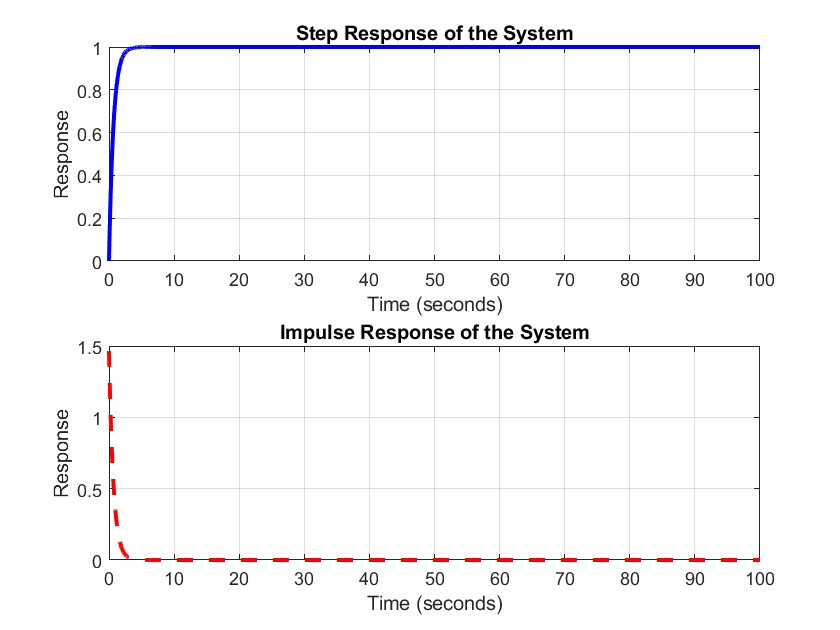
\includegraphics[width=0.7\textwidth]{eunsoo/E-1-4-step-and-impulse.jpg}
    \hfill
    \caption{The step and impulse responses of the plant}
    \label{figure:E-1-4-step-and-impulse}
\end{figure}

\vspace{-10mm}
\subsubsection{Discussion}
- (D) discussion of how my choices led to better achievement of the final objectives, compared to other control strategies

% TESTING WHERE TO PUT BIBLIOGRAPHY
% \begingroup\onehalfspacing
% {\small
% %\renewcommand{\section}[2]{}
% \begin{multicols}{2}
% \bibliographystyle{unsrt}
% %\bibliographystyle{elsarticle-num}
% % \bibliographystyle{elsarticle-harv}
% % \bibliographystyle{elsarticle-num-names}
% % \bibliographystyle{model1a-num-names}
% % \bibliographystyle{model1b-num-names}
% % \bibliographystyle{model1c-num-names}
% % \bibliographystyle{model1-num-names}
% % \bibliographystyle{model2-names}
% % \bibliographystyle{model3a-num-names}
% % \bibliographystyle{model3-num-names}
% % \bibliographystyle{model4-names}
% % \bibliographystyle{model5-names}
% % \bibliographystyle{model6-num-names}
% \bibliography{mybib.bib}
% \end{multicols}}
% \endgroup
\setlength{\headheight}{13.6pt}
\addtolength{\topmargin}{-1.6pt}
\newpage
\subsection{Oxygen control}
\setlength{\headheight}{13.6pt}
\addtolength{\topmargin}{-1.6pt}
\newpage
\subsection{Acidity control}

\setlength{\headheight}{13.6pt}
\addtolength{\topmargin}{-1.6pt}
\newpage
\section{Purification methods}
\subsection{Lactic acid purification}

\fancyhead[L]{}
\fancyhead[R]{PURIFICATION METHODS - EUNSOO CHANG}
\clearpage
\newpage
\subsection{Ammonia purification}

\setlength{\headheight}{13.6pt}
\addtolength{\topmargin}{-1.6pt}
\newpage
\section{Final product formulation}
\fancyhead[L]{}
\fancyhead[R]{FINAL PRODUCT FORMULATION - EUNSOO CHANG}
\clearpage


\newpage
\thispagestyle{nullheader}

%\begingroup\onehalfspacing
%{\small
%\renewcommand{\section}[2]{}
%\begin{multicols}{2}
%\bibliographystyle{plain}
%\bibliographystyle{elsarticle-num}
% \bibliographystyle{elsarticle-harv}
% \bibliographystyle{elsarticle-num-names}
% \bibliographystyle{model1a-num-names}
% \bibliographystyle{model1b-num-names}
% \bibliographystyle{model1c-num-names}
% \bibliographystyle{model1-num-names}
% \bibliographystyle{model2-names}
% \bibliographystyle{model3a-num-names}
% \bibliographystyle{model3-num-names}
% \bibliographystyle{model4-names}
% \bibliographystyle{model5-names}
% \bibliographystyle{model6-num-names}
%\bibliography{mybib}
%\end{multicols}}
%\endgroup
\printbibliography

\end{document}